%!TEX root=./Emile.tex
\subsection[Netzwerktheorie]{Menschliches Zusammenleben - eine Welt voller Verbindungen}

\epigraph{
	``Wer da hat dem wird gegeben, dass er die Fülle habe; wer aber nicht hat, dem wird genommen, was er hat.''\\*
	\emph{Matthäus, 25, 29}
}

Um Netzwerke, Systeme von Verbindungen zwischen Entitäten, theoretisch betrachten und analysieren zu können, gibt es die Möglichkeit sie als Graph darzustellen \parencite[vgl.]{Kleinberg-2009-oz}.
Dabei gibt es Kanten und Knotenpunkte.
Knotenpunkte können untereinander durch Kanten verbunden werden, die soziale Verbindung, Bekanntschaft, gemeinsame Arbeiten etc. darstellen.
Ein Beispiel für Netzwerke, die mit Graphen dargestellt werden können, sind beispielsweise die Deutsche Schülerakademie, bei der jeder Knoten einen Teilnehmer repräsentiert, der mit verschiedenen anderen in Beziehung steht (dargestellt durch Kanten).
Genauso kann man auch Beziehungen in einer Lerngruppe wie einer Schulklasse oder andere Netzwerke graphisch darstellen.

\begin{figure}[htbp]
	\begin{center}
	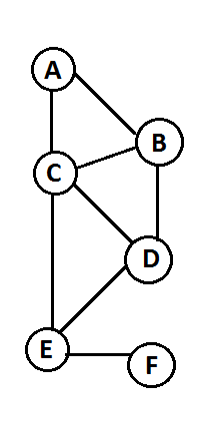
\includegraphics[width=1\textwidth]{img\graph1.png}
	\caption{Beispiel für die Darstellung eines Graphen \cite{Kleinberg-2009-oz}}
	\label{fig:graph1}
	\end{center}
\end{figure}

Innerhalb der Struktur des Graphs kann es Besonderheiten, wie z.B. Komponente geben, einzelne Netzwerke, welche nicht über einen Pfad mit jedem anderen Knoten im Graph verbunden sind.

\begin{figure}[htbp]
	\begin{center}
	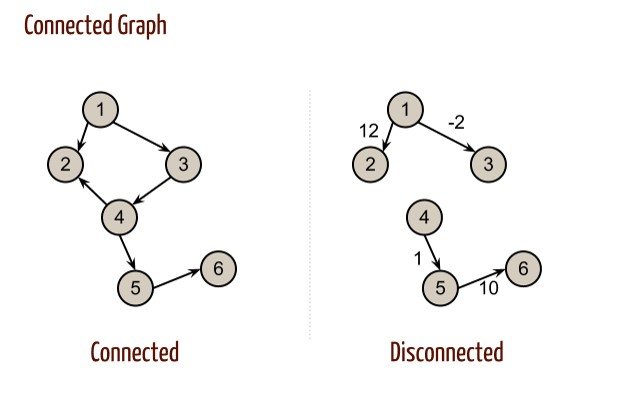
\includegraphics[width=1\textwidth]{img\Graph-Connected.jpg}
	\caption{Beispiel für unverbundene Graphen \cite{Kleinberg-2009-oz}}
	\label{fig:graph1}
	\end{center}
\end{figure}


\subsubsection{Schlussfolgerungen aus der Netzwerktheorie}

Aus dieser Ausgangssituation kann man je nach Betrachtungsweise verschiedene Schlussfolgerungen ziehen.
Beispielsweise kann man den Informationsfluss in Netzwerken analysieren.

\paragraph{Kaskaden und Cluster}

Mithilfe von Graphen ist es möglich, Die Ausbreitung von Ideen oder Technologien innerhalb eines Netzwerks zu beschreiben.
Laut Kleinberg ist diese Verbreitung von sozialen Gründen abhängig, Menschen entscheiden sich aufgrund ihrer sozialen Nachbarn.
Hierbei geht man von einer bestimmten Anzahl von Subjekten (also Knoten) aus, die diese Neuerung benutzen.
Ihre Nachbarn werden dann nacheinander entscheiden, ob sie diese übernehmen möchten oder nicht, dies wird entschieden durch einen \emph{Treshold} (Grenze), die angibt, welcher Anteil von Nachbarn die Neuerung mindestens benutzen müssen, damit man diese auch übernimmt.
Dementsprechend findet eine Ausbreitung durch das Netzwerk, eine Kaskade, statt.
Diese wird in einigen Fällen gestoppt, endet also, ohne das gesamte Netzwerk übernommen zu haben.
Liegt das Treshold für eine NEuerung beispielsweise bei 0,4 , müssen also mindestens 2/5 der Nachbarn von Knoten \emph{X} diese Neuerung benutzen, damit sie übernommen wird.
Wenn \emph{X} aber vier Nachbarn hat, von denen nur einer die Neuerung hat, ist eine Veränderung für \emph{X} nicht attraktiv genug, es sei denn, ein anderer Nachbar entscheidet sich auch um.
Gehen wir aber davon aus, dass alle anderen Nacbarn von \emph{X} nur untereinander verbunden sind und einen eigenen Abschnitt des Netzwerks bilden und somit nur über \emph{X} ein Pfad zu anderen besteht, gibt es keine Möglichkeit für \emph{X}, das Treshold zu erreichen, es kommt zum Ausbreitungsstopp.
Diese Abschnitte innerhalb von Netzwerken bezeichnet man als \emph{Cluster}, also Bereiche des Netzwerks mit eng untereinander verbundenen Knoten, die allerdings nur wenige Verbindungen zu Knoten außerhalb des Clusters haben.
An den Grenzen dieser Cluster terminiert die Kaskade einer Neuerung, da der Treshold für Außenstehende nicht erfüllt werden kann.
Eine eng verbundene Gruppe innerhalb eines Netzwerks sorgt also für eine \emph{Isolation} einer Neuerung von anderen Teilen des Netzwerks.
Besonders deutlich wird dies beispielsweise beim Sprachgebrauch und Vokabular innerhalb der Schülerakademie;
So gehören Begriffe wie KüA oder AKL in der DSA zum normalen Sprachgebrauch und sind bei allen Teilnehmern etabliert, sie werden sich allerdings kaum darüber hinaus in den Wortschatz ausbreiten, da die DSA einen eigenen, von anderen Bereichen isolierten Kontext darstellt.
Die Netzwerktheorie macht somit deutlich, weshalb bestimmte gemeinsam geteilte Angewohnheiten oder Neuerungen sich nur in einem bestimmten Cluster etablieren und somit große Netzwerke in kleinere Abschnitte unterteilen, die wiederum in ihren Eigenschaften mehr oder weniger unabhängig und isoliert voneinander bestehen.
Diese relative Isolation kann in bestimmten Fällen sowohl einen Vorteil der Mitglieder innerhalb der Gruppe als auch eine Abgrenzung von Außenstehenden zur Folge haben, da diese keine Möglichkeit haben, Neuerungen der Gruppe zu übernehmen.

\paragraph{Bezüge zu Zimpel}

Eine Anwendung in der Pädagogik bietet\citeauthor{Zimpel2012}, der in seinem Text als ein ein zentrales Problem des Lehrens in der Schule die Heterogenität in einer Lerngruppe beschreibt, durch die ein Konflikt zwischen der Möglichkeit einer individuellen Förderung und dem Ziel eines gemeinsamen Lernens, das jeden Schüler in gleicher Weise berücksichtigt, besteht.
Die Lehrenden müssen sich also der Frage stellen, welches der beiden Ziele, Individualität oder Gemeinschaft, auf Kosten des anderen stärker verfolgt werden soll.
\citeauthor{Zimpel2012} stellt drei Möglichkeiten vor:
Ein Prinzip, bei dem die Individualität des Einzelnen in den Vordergrund gestellt wird, ist das \emph{Matthäusprinzip}.
Sein Grundsatz sagt aus: "„Wer viel hat, dem wird viel gegeben; wer wenig hat, dem wird genommen“ \parencite[105]{Zimpel2012}.
Man kann es damit erklären, dass Menschen mit \emph{mehr} (zum Beispiel Begabung oder Geld) bessere Voraussetzungen haben und automatisch leichter *noch mehr* erreichen als andere mit  \emph{weniger}, wodurch sich die Unterschiede verstärken.
Oft findet dies auch bewusst in Form von gezielter Förderung und speziellen Programmen für leistungsstarke Schüler wie beispielsweise der DSA statt.
Diese leistungsstarken Schüler bilden dann in der Gesamtschülerschaft ein eigenes Cluster, durch das sie sich von den anderen leistungsschwächeren Schülern abgrenzen. Sie bekommen so Zugang zu speziellen Inhalten, Methoden oder auch wichtigen Kontakten und Möglichkeiten, von denen sie untereinander profitieren, zu denen schwächere Schüler aber keinen Zugang finden können.
Zum einen entstehen dadurch größere gesellschaftliche und schulische Disparitäten, andererseits bietet sich aufgrund der verschiedenen Fähigkeitsstufen eine Wettbewerbssituation, die als Motivation für schwächere dienen kann.

\emph{Das Normalisierungsprinzip} kann als Gegenstück des Matthäusprinzips betrachtet werden: ``Wer wenig hat, bekommt. Wer viel hat, gibt.'' \parencite[12]{Zimpel2012}.
Durch verschiedene Maßnahmen wird hier ein Ausgleich angestrebt.
Die Anzahl der Schüler, die dem Mittelmaß zugeordnet werden können, steigen demnach an, extreme Abweichungen nehmen entsprechend ab.
Besonders in der Sonderpädagogik wird dieses System häufig angewendet, um benachteiligten Schülern gleiche Chancen einzuräumen.
Als Netzwerk dargestellt, gäbe es beim Normalisierungsprinzip keine Cluster oder Abgrenzungen, da jeder Schwache mit starken Schülern in Kontakt steht.
Das Ideal dieses Prinzips wäre eine Lerngruppe, in der ein homogener Bildungsstandard herrscht.
In der Netzwerktheorie stößt das Prinzip allerdings schon an seine Grenzen, wenn man Personen am Rand des Netzwerks betrachtet, die zwangsläufig weniger Kontakte als andere haben.

Da diese beiden Prinzipien, werden sie als einziges und vollständig angewendet, gravierende Nachteile mit sich bringen, stellt \citeauthor{Zimpel2012} eine dritte Möglichkeit vor, wie die beschriebenen Probleme didaktisch gelöst werden könnten: den \emph{Hyperzyklus}.
Dieses Prinzip erläutert, wie Integration als Balance zwischen Anerkennung von Individualität und Gleichwertigkeit aller Schüler gelingen kann.
Der didaktische Hyperzyklus beruht darauf, dass sich alle Schüler als hilfreich für andere erleben können.
So entsteht ein rekursives, zirkuläres System von gegenseitiger Hilfestellung (Rot hilft Gelb, Gelb hilft Grün, Grün hilft Rot, etc.).
Es entsteht ein ``Fluss des Gebens und Nehmens'' \parencite[125]{Zimpel2012}, bei dem, trotz der unterschiedlichen Voraussetzungen der Schüler, alle in den Lernprozess eingebunden werden konnten.

Auch beim Hyperzyklus gibt es dementsprechend keine Clustergrenzen und somit keine Abgrenzung zwischen Schülern verschiedener Leistungsstärken.
Das Prinzip kategorisiert nicht zwangsläufig in stark oder schwach, sondern differenziert den Leistungsbegriff und berücksichtigt viele verschiedene Fähigkeiten und Begabungen.
Somit kann jeder Schüler als Hilfe dienen und Hilfe empfangen.

\paragraph{Power Law}

Wie sich bereits mithilfe der Graphen- und Netzwerktheorie erklären ließ, hat jeder Mensch innerhalb eines Netzwerks einen bestimmten klar definierten Bekanntenkreis aller mit ihm verbundenen Nachbarn.
Dieser ist in der Realität in den meisten Fällen zahlenmäßig überschaubar, allerdings gibt es Ausnahmen von prominenten Personen, deren Bekanntheit über ihren direkten Bekanntenkreis hinausgeht, in manchen Fällen (z.B. Barack Obama) kommt es sogar zu globaler Bekanntheit.
Das selbe Phänomen erkennen wir bei anderen Medien, die Popularität erlangen können, wie Musik, Bücher, etc.
Daraus ergibt sich für Kleinberg die grundlegende Fragestellung:
Wenn jeder Mensch einen messbaren Bekanntheitsgrad \emph{k} besitzt, wie lässt sich die Verteilung der verschiedenen \emph{k} in der Gesamtbevölkerung als Funktion modellieren?
Einen naheliegenden Ansatz stellt die Normalverteilung dar, welche bei vielen Phänomenen in der Natur Anwendung findet. Hierbei scharen sich die Anteile um einen Mittelwert und sinken für größere und kleinere \emph{k} exponentiell ab.
Ein anderer Ansatz ist das \emph{Power Law}.
Kleinberg bringt hierbei das Beispiel von Internetseiten, modelliert man für diese die Verteilung der Bekanntheiten, ergibt sich eine hyperbelförmige Kurve mit der Funktion \emph{1/k²}.
 Wertet man die Daten mehrerer Verteilungen aus, so zeigt sich, dass das Power Law im Großteil der Fälle überwiegt, wenn auch die Funktionen sich in ihren Parametern leicht unterscheiden (So zum Beispiel \emph{1/k³} bei Romanen).
Allerdings gilt für alle die allgemeine Gleichung des Power Law:
\emph{f(k) = a/(k^c)}
Der Vorteil dieses Modells und der Unterschied zur Normalverteilung besteht im Verhalten des Graphen für große \emph{k}:
Während die Anteile bei exponentieller Abnahme mit steigendem \emph{k} gegen Null streben, sinkt die Kurve beim Power Law deutlich langsamer, was bedeutet, dass die Werte für hohe \emph{k} deutlich größer sind und dass auch höhere Werte für \emph{k} erreicht werden können. In der Praxis erklärt dieses Modell damit gut das Zustandekommen von Prominenz und Berühmtheit sowie das Auftreten in extremer Ausprägung, bei der einzelneMenschen fast uneingeschränkte globale Popularität erlangen können.
